\chapter{Autonomous navigation of micro-magnetic rollers} \footnotetext{This chapter is adapted from unpublished work}
\section{Introduction}


\section{Experiment}
The same setup is adapted from our group's previous paper as shown in \textcolor{red}{fig xxx}. \cite{fei2018magneto, fei2019magneto} A 3 dimensional time variance magnetic field is generated with a three axis electric magnetic coil mounted on the microscope. The orientation of magnetic field is controlled by the wave functioned in $x$, $y$ and $z$ direction. The magnitude of magnetic field is controlled by the current. The field can be rotated by multiply a 3-d rotational matrix. 3D printed  surfaces with slope angle from $5^o$ to  $10^o$ are put under microscope to generate gravity field. 
\section{Result and discussion}
\begin{figure}[p]
\centering
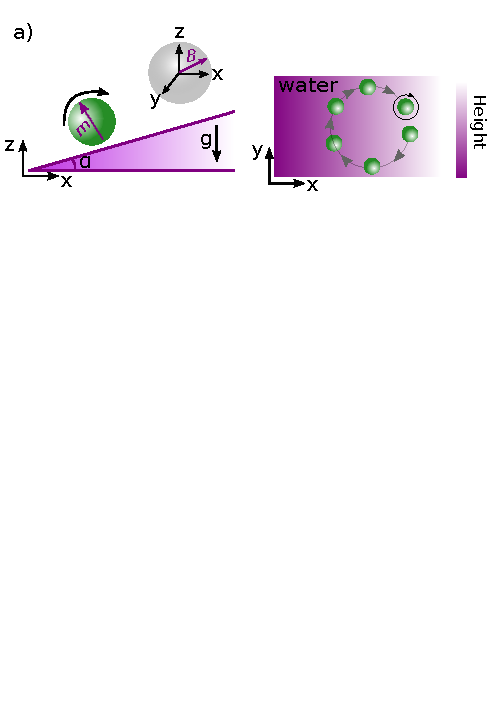
\includegraphics[width=9cm]{figures/5_1.pdf}
\caption{ (a) Schematic illustration of a magnetic micro particles rolling on a horizontal and inclined surface in a 3 dimensional magnetic field.(b) Microscope image of  micro particles motions on a horizontal surface and inclined surface. Here, the radius of micro particle is 33.9 $\mu mu$ }
\label{fig:1}
\end{figure}
\section{Modelling }
We consider a magnetic sphere with radius $a$ and permanent magnetic moment $\ve{m}$ moving through a viscous fluid at a fixed height above a solid plane under the influence of a time-varying magnetic field $\ve{B}(t)$. In a uniform field, the particle experiences a magnetic torque, $\ve{L}_{\m}=\ve{m}\times\ve{B}(t)$, but no magnetic force, $\ve{F}_{\m}=0$. In the absence of inertial effects (i.e., at low Reynolds number), the magnetic force and torque on the particle are balanced by the hydrodynamic force and torque, which are linearly related to the particle's linear velocity $\ve{U}$ and angular velocity $\ve{\Omega}$ as
\begin{equation}
    \begin{bmatrix} \ve{F}_{\m} \\ \ve{L}_{\m} \end{bmatrix} = \begin{bmatrix} \ve{A} & \ve{\tilde{B}} \\ \ve{B} & \ve{C} \end{bmatrix}  \cdot \begin{bmatrix} \ve{U} \\ \ve{\Omega} \end{bmatrix} \label{eq:dynamics}
\end{equation}
where $\ve{A}$, $\ve{B}$, $\ve{\tilde{B}}$, and $\ve{C}$ are components of the hydrodynamic resistance tensor.  For a solid sphere above a solid plane normal to the $z$-direction, the components of the resistance tensor have the form
\begin{align}
    \ve{A} &=  6\pi \eta a \begin{bmatrix} 
        Y_A & \cdot & \cdot \\
        \cdot & Y_A & \cdot \\
        \cdot & \cdot & X_A  \end{bmatrix}
    \\
    \ve{B}=-\ve{\tilde{B}}&= 6\pi \eta a^2 \begin{bmatrix} 
        \cdot & Y_B & \cdot \\
        -Y_B & \cdot & \cdot \\
        \cdot & \cdot & \cdot  \end{bmatrix}
    \\
    \ve{C} &- 6\pi \eta a^3 \begin{bmatrix} 
        Y_C & \cdot & \cdot \\
        \cdot & Y_C & \cdot \\
        \cdot & \cdot & X_C  \end{bmatrix} 
\end{align}
where $\eta$ is the fluid viscosity. The coefficients $Y_A$ and $Y_B$ describe, respectively, the dimensionless force and torque on a sphere translating parallel to a solid planar surface.\autocite{ONeill1964a} The coefficient $Y_C$ describes the torque on a sphere rotating about an axis parallel to the surface.\autocite{Dean1963} The coefficient $X_A$ describes the force on a sphere translating perpendicular to the surface \autocite{Brenner1961a}.  Finally, $X_C$ describes the torque on a sphere rotating about an axis perpendicular to a the surface. \autocite{Jeffrey1915} These coefficients depend only on the surface separation $\delta$ scaled by the particle radius $a$ as illustrated in Figure \ref{fig:resistance}.

Substituting the above expressions for the resistance tensor, the linear velocity $\ve{U}$ and angular velocity $\ve{\Omega}$ can be expressed explicitly in terms of the magnetic torque as
\begin{align}
    6\pi\eta a^2 \ve{U} &= \frac{Y_A}{Y_A Y_C - Y_B^2}\begin{bmatrix} 
        \cdot & -\kappa & \cdot \\
        \kappa & \cdot & \cdot \\
        \cdot & \cdot & \cdot  \end{bmatrix} \cdot \ve{L}_{\m} \label{eq:U}
    \\
    6\pi\eta a^3 \ve{\Omega} &= \frac{Y_A}{Y_A Y_C - Y_B^2}\begin{bmatrix} 
        1 & \cdot & \cdot \\
        \cdot & 1 & \cdot \\
        \cdot & \cdot & \lambda  \end{bmatrix} \cdot \ve{L}_{\m} \label{eq:W}
\end{align}
where $\kappa = Y_B/Y_A$ and $\lambda=(Y_A Y_C -Y_B^2)/(Y_A X_C)$. These dynamics imply that the particle velocity normal to the planar substrate is identically zero (i.e., $U_z=0$). We therefore assume that the surface separation $\delta$ and the resistance coefficients are constant throughout the particle's dynamics. 

%%%%%%%%%%%%%%%%%%%%%%%%%%%%%%%%%%
\subsection*{Non-dimensionalization}

To facilitate both numerical solution and analytical analysis of the particle dynamics, it is convenient to introduce dimensionless variables using the following scales
\begin{align}
    \text{magnetic field: } & B_0
    \\
    \text{torque: } &  mB_0
    \\
    \text{length: } & a
    \\
    \text{time: } & \frac{6\pi \eta a^3 (Y_A Y_C-Y_B^2)}{m B_0 Y_A}  
\end{align}
In dimensionless form, the dynamical equations (\ref{eq:U}) and (\ref{eq:W}) depend on the  two constant parameters $\kappa$ and $\lambda$ along with the time-varying magnetic field $\ve{B}(t)$. Below, we use the same notation to refer to dimensionless quantities, which corresponds to setting the characteristic scales to unity in the dynamical equations (\ref{eq:U}) and (\ref{eq:W}) (e.g., $a\rightarrow 1$).

%%%%%%%%%%%%%%%%%%%%%%%%%%%%%%%%%%
\subsection{Numerical Solution (Unit Quaternion)}

The dynamics of equations (\ref{eq:U}) and (\ref{eq:W}) are solved numerically to determine the particle position $\ve{x}_{\p}(t)$ and its orientation parameterized by the unit quaternion $\ve{q}(t)=[q_0,q_1,q_2,q_3]^T$. At each point in time, the magnetic torque $\ve{L}_{\m}$ expressed in the world coordinate system of the substrate depends on the particle orientation as
\begin{equation}
    \ve{L}_m = (R(\ve{q})^T\ve{m}')\times \ve{B}(t) \label{eq:Lm}
\end{equation}
where $\ve{m}'=[0,0,1]^T$ is the constant magnetic moment expressed in the body-fixed coordinate system of the particle, and $R(\ve{q})$ is an orthogonal rotation matrix\autocite{Diebel2006} defined as
\begin{equation}
    R(\ve{q}) = \begin{bmatrix}
    q_0^2 + q_1^2 - q_2^2 - q_3^2 & 2q_1q_2 + 2q_0q_3 & 2q_1q_3 - 2q_0q_2 \\
    2q_1q_2 - 2q_0q_3 & q_0^2 - q_1^2 + q_2^2 - q_3^2 & 2q_2q_3 + 2q_0q_1 \\
    2q_1q_3 + 2q_0q_2 & 2q_2q_3 - 2q_0q_1 & q_0^2 - q_1^2 - q_2^2 + q_3^2
    \end{bmatrix}
\end{equation} 
Given the torque $\ve{L}_{\m}$, the linear velocity $\ve{U}$ and angular velocity $\ve{\Omega}$ are given by equations (\ref{eq:U}) and (\ref{eq:W}). Starting from some initial conditions $\ve{x}_p(0)$ and $\ve{q}(0)$, the position and orientation evolve in time as 
\begin{align}
    \dot{\ve{x}_p} &= \ve{U} \label{eq:position}
    \\
    \dot{\ve{q}} &= \frac{1}{2}W(\ve{q})^T \ve{\Omega} \label{eq:orientation}
\end{align}
where the $3\times4$ matrix $W(\ve{q})$ is defined as 
\begin{equation}
    W(\ve{q}) = \begin{bmatrix}
    -q_1 & q_0 & -q_3 & q_2 \\
    -q_2 & q_3 & q_0 & -q_1 \\
    -q_3 & -q_2 & q_1 & q_0
    \end{bmatrix}
\end{equation}
Equations (\ref{eq:position}) and (\ref{eq:orientation}) are integrated numerically in \emph{Mathematica}.


%%%%%%%%%%%%%%%%%%%%%%%%%%%%%%%%%%
\subsection*{Numerical Solution (Euler Angles)}

Alternatively, the orientation of the particle can be parameterized by the Euler angles $\ve{u}=[\phi,\theta,\psi]^T$ with rotation matrix\autocite{Diebel2006}
\begin{equation}
    R_{313}(\ve{u}) = \begin{bmatrix} 
     c_\phi c_\psi -  s_\phi c_\theta s_\psi  &  c_\phi s_\psi + s_\phi c_\theta c_\psi  &  s_\phi s_\theta \\
   -s_\phi c_\psi  - c_\phi c_\theta s_\psi &  -s_\phi s_\psi + c_\phi  c_\theta c_\psi &  c_\phi s_\theta  \\
    s_\theta s_\psi  & - s_\theta c_\psi  & c_\theta  \end{bmatrix}
\end{equation}
with $c_x =\cos(x)$ and $s_x=\sin(x)$. This rotation matrix can be substituted into equation (\ref{eq:Lm}) to express the magnetic torque in terms of the Euler angles. The Euler angle rates $\dot{\ve{u}}$ depend on the angular velocity $\ve{\Omega}$ in the world coordinate system as 
\begin{equation}
    \dot{\ve{u}} = E_{313}^{-1}(\ve{u})~ \ve{\Omega}
\end{equation}
wehere the matrix $ E_{313}^{-1}(\ve{u})$ is \begin{equation}
    E^{-1}_{313}(\ve{u}) = \frac{1}{s_{\theta}}\begin{bmatrix} 
     s_{\psi} & -c_{\psi} & 0
     \\
     s_{\theta} c_{\psi} & s_{\theta} s_{\psi} & 0
     \\
     -s_{\psi}c_{\theta} & c_{\psi}c_{\theta} & s_{\theta}
     \end{bmatrix}
\end{equation}
The resulting dynamical equations for the particle orientation can be simplified as
\begin{align}
    \dot{\phi} &= h(\theta,\psi) = -\cot \theta (B_x\cos\psi +B_y\sin\psi)
    \\
    \dot{\theta} &= f(\theta,\psi) = -\cos\theta (B_y \cos\psi - B_x \sin\psi) - B_z\sin\theta \label{eq:theta}
    \\
    \dot{\psi} &= g(\theta,\psi) = \tfrac{1}{2} \left((1+\lambda) +(1-\lambda)\cos2\theta \right) \csc\theta (B_x \cos \psi + B_y\sin\psi ) \label{eq:psi}
\end{align}
Note that the dynamics of the angles $\theta$ and $\psi$ can be solved independently of $\phi$.  This simplification follows from the fact that there is no torque on the particle about the axis of its magnetic moment. Similarly, the particle velocity in the plane of the substrate can be expressed as
\begin{align}
    U_x = \kappa (B_x \cos \theta -  B_z \sin \psi \sin\theta) \label{eq:Ux}
    \\
    U_y = \kappa (B_y \cos\theta + B_z \cos\psi \sin\theta ) \label{eq:Uy}
\end{align}
Equations (\ref{eq:theta})--(\ref{eq:Uy}) are integrated numerically to determine the motion of the particle in the prescribed magnetic field $\ve{B}(t)$.
\subsection*{Numerical Solution (Euler Angles)}

Alternatively, the orientation of the particle can be parameterized by the Euler angles $\ve{u}=[\phi,\theta,\psi]^T$ with rotation matrix\autocite{Diebel2006}
\begin{equation}
    R_{313}(\ve{u}) = \begin{bmatrix} 
     c_\phi c_\psi -  s_\phi c_\theta s_\psi  &  c_\phi s_\psi + s_\phi c_\theta c_\psi  &  s_\phi s_\theta \\
   -s_\phi c_\psi  - c_\phi c_\theta s_\psi &  -s_\phi s_\psi + c_\phi  c_\theta c_\psi &  c_\phi s_\theta  \\
    s_\theta s_\psi  & - s_\theta c_\psi  & c_\theta  \end{bmatrix}
\end{equation}
with $c_x =\cos(x)$ and $s_x=\sin(x)$. This rotation matrix can be substituted into equation (\ref{eq:Lm}) to express the magnetic torque in terms of the Euler angles. The Euler angle rates $\dot{\ve{u}}$ depend on the angular velocity $\ve{\Omega}$ in the world coordinate system as 
\begin{equation}
    \dot{\ve{u}} = E_{313}^{-1}(\ve{u})~ \ve{\Omega}
\end{equation}
wehere the matrix $ E_{313}^{-1}(\ve{u})$ is \begin{equation}
    E^{-1}_{313}(\ve{u}) = \frac{1}{s_{\theta}}\begin{bmatrix} 
     s_{\psi} & -c_{\psi} & 0
     \\
     s_{\theta} c_{\psi} & s_{\theta} s_{\psi} & 0
     \\
     -s_{\psi}c_{\theta} & c_{\psi}c_{\theta} & s_{\theta}
     \end{bmatrix}
\end{equation}
The resulting dynamical equations for the particle orientation can be simplified as
\begin{align}
    \dot{\phi} &= h(\theta,\psi) = -\cot \theta (B_x\cos\psi +B_y\sin\psi)
    \\
    \dot{\theta} &= f(\theta,\psi) = -\cos\theta (B_y \cos\psi - B_x \sin\psi) - B_z\sin\theta \label{eq:theta}
    \\
    \dot{\psi} &= g(\theta,\psi) = \tfrac{1}{2} \left((1+\lambda) +(1-\lambda)\cos2\theta \right) \csc\theta (B_x \cos \psi + B_y\sin\psi ) \label{eq:psi}
\end{align}
Note that the dynamics of the angles $\theta$ and $\psi$ can be solved independently of $\phi$.  This simplification follows from the fact that there is no torque on the particle about the axis of its magnetic moment. Similarly, the particle velocity in the plane of the substrate can be expressed as
\begin{align}
    U_x = \kappa (B_x \cos \theta -  B_z \sin \psi \sin\theta) \label{eq:Ux}
    \\
    U_y = \kappa (B_y \cos\theta + B_z \cos\psi \sin\theta ) \label{eq:Uy}
\end{align}
Equations (\ref{eq:theta})--(\ref{eq:Uy}) are integrated numerically to determine the motion of the particle in the prescribed magnetic field $\ve{B}(t)$.

%%%%%%%%%%%%%%%%%%%%%%%%%%%%%%%%%%
\subsection{Two-Timing Perturbation Solution}

For time-periodic magnetic fields of frequency $\omega$, the particle dynamics can be approximated using the following perturbation expansion based on \emph{two-timing}.\autocite{Strogatz2015} Here, the dimensionless quantity $6\pi \eta a^3 \omega (Y_A Y_C - Y_B^2)/m B_0 Y_A$ is the small parameter, which we denote simply as $\omega$ in the dimensionless formulation. This quantity represents the ratio between the applied frequency and the relaxation rate at which the particle aligns with the field.  Our assumption that $\omega\ll 1$ implies that relaxation is fast relative to the driving field, such that the particle's magnetic moment aligns closely with the field. Under these conditions, we introduce two time variables: a slow time $T=\omega t$ corresponding to the driving field and a fast time $\tau=t$ corresponding to the particle relaxation.  The solution to equations (\ref{eq:theta}) and (\ref{eq:psi}) can then be expanded as
\begin{align}
    \theta(t,\omega) &= \theta_0(\tau,T) + \omega \theta_1(\tau,T) + \omega^2 \theta_2(\tau,T) + O(\omega^3) \label{eq:thetaPower}
    \\
    \psi(t,\omega) &= \psi(\tau,T) + \omega \psi_1(\tau,T) + \omega^2 \psi_2(\tau,T) + O(\omega^3) \label{eq:psiPower}
\end{align}
Substituting these expansions into the governing equations and collecting like powers in $\omega$, we obtain a hierarchy of perturbation equations that can be solved sequentially. We are primarily interested in the slow time dynamics of the particle over one cycle of the oscillation period; we therefore focus on the limit as $\tau\rightarrow\infty$ in which the fast relaxation processes have fully equilibrated.

At the periodic steady-state, the displacement $\ve{\Delta}$ of the particle during one oscillation cycle is given by the following integral of the slow time over one oscillation cycle
\begin{equation}
    \ve{\Delta} = \int_0^{2\pi} \ve{U}(T) dT
\end{equation}
where the components of the velocity are given by equations (\ref{eq:Ux}) and (\ref{eq:Uy}).  Substituting the perturbation expansions (\ref{eq:thetaPower}) and (\ref{eq:psiPower}), the velocity and the displacement can be expanded as
\begin{align}
    \ve{U} &= \omega \ve{U}_1 + \omega^2 \ve{U}_2 + O(\omega^3)
    \\
    \ve{\Delta} &= \omega \ve{\Delta}_1 + \omega^2 \ve{\Delta}_2 + O(\omega^3)
\end{align}
Note that the zeroth order contributions are identically zero as there is no motion in the limit of zero frequency. Below, we derive expressions for the first and second order displacements as a function of the applied field $\ve{B}(T)$.

%%%%%%%%%%%%%%%%%%%%%%%%%%%%%%%%%%
\subsubsection*{Zeroth Order, $O(\omega^0)$}

The zeroth order equations are 
\begin{align}
    \partial_{\tau} \theta_0 = f(\theta_0,\psi_0)
    \\
    \partial_{\tau} \psi_0 = g(\theta_0,\psi_0)
\end{align}
After some time of $O(1)$, the time derivatives relax to zero (e.g., $\partial_{\tau} \theta_0\rightarrow 0$), and the orientation of the particle is specified by the applied field. The resulting solution is 
\begin{align}
    \theta_0(\infty,T) &= \mathrm{atan2}((B_x^2+B_y^2)^{1/2},B_z) \label{eq:theta0}
    \\
    \psi_0(\infty,T) &= \mathrm{atan2}(B_x,-B_y) \label{eq:psi0}
\end{align}
where $\mathrm{atan2}(y,x)$ is the 2-argument arctangent function. Note that the components of the applied field depend on the slow time (e.g., $B_x = B_x(T)$).

\section{Designing the Magnetic Field}

\begin{equation}
    \begin{bmatrix} 0 \\ \ve{m}\times\ve{B} \end{bmatrix} = \mathcal{R} \cdot \begin{bmatrix} \ve{U} \\ \ve{\Omega} \end{bmatrix} \label{eq:dynamics}
\end{equation}

The time-average velocity is 
\begin{align}
    \hat{U}_x &= \omega \hat{U}_x^{(1)}+\omega^2 \hat {U}_x^{(2)} + O(\omega^3) 
    \\
    \hat{U}_y &= \omega \hat{U}_y^{(1)} + \omega^2 \hat {U}_y^{(2)} + O(\omega^3) 
\end{align}
if there is a slope of angle $\phi$ in the $x$-direction then
\begin{align}
    \hat{U}_x^{(1)} &= 0 
    \\
    \hat {U}_x^{(2)} &\propto \phi + O(\phi^2)
\end{align}

\begin{equation}
    \ve{B}(t) = B \cos(\omega t) \ve{e}_x + B \sin (\omega t) \ve{e}_y
\end{equation}

\begin{align}
    \hat{U}_x &= 0 + O(\omega^2) 
    \\
    \hat {U}_y &= - C a \omega \alpha + O(\alpha^2) + O(\omega^2) 
\end{align}

\begin{align}
    \hat{U}_x &= a\omega \alpha\left( 0  + D_x \frac{\lambda \omega}{m B}\right) + \dots
    \\
    \hat {U}_y &= a\omega \alpha\left(C_y  + D_y \frac{\lambda\omega}{m B} \right) + \dots
\end{align}

\begin{align}
    \hat{U}_y^{(1)} &\propto \phi + O(\phi^2) 
    \\
    \hat {U}_y^{(2)} &\propto \phi + O(\phi^2)
\end{align}
\begin{equation}
    \hat{U}_y = 0
\end{equation}
where 
\begin{equation}
    \omega = \frac{\lambda\omega}{m B}
\end{equation}

Rotational Symmetry
\begin{equation}
    R_z(\tfrac{2\pi}{m}) \ve{B}(\omega t) = \ve{B}(\omega t - \tfrac{2\pi}{m}) 
\end{equation}




 \section{Design the Magnetic Field}
 We consider periodic magnetic fields $\ve{B}(t)$ with a fundamental frequency $\omega$ and $N$ harmonics
\begin{equation}
    \ve{B}(t) = \tfrac{1}{2} \ve{a}_0 + \sum_{n=1}^N \ve{a}_n \cos(n\omega t) + \ve{b}_n \sin(n\omega t)
\end{equation}
where $\ve{a}_n$ and $\ve{b}_n$ are constant vectors. This $6N+3$ dimensional design space is constrained by additional requirement that the field have $m$-fold rotational symmetry about the $z$-axis
\begin{equation}
    R_z(\varphi_m) \ve{B}(\omega t) = \ve{B}(\omega t - \varphi_m) \label{eq:symmetry}
\end{equation}
where $\varphi_m=2\pi/m$ for positive integer $m\geq 3$, and $R_z(\varphi)$ is the following rotation matrix about the $z$-axis
\begin{equation}
    R_z(\varphi) = \begin{bmatrix} 
    \cos \varphi & \sin \varphi & 0 \\
    -\sin \varphi & \cos \varphi & 0 \\
    0 & 0 & 1    
    \end{bmatrix}
\end{equation}
For $n=0$, equation (\ref{eq:symmetry}) implies that $\ve{a}_0 = a_0 \ve{e}_z$. For $n\geq1$, equation (\ref{eq:symmetry}) has terms like $\cos(n \omega t)$ and $\sin(n\omega t)$, which can be collected to give six linear equations for the six coefficients 
\begin{equation}
    \begin{bmatrix} 
    R_z(\varphi_m) - I \cos(n\varphi_m) & I \sin(n \varphi_m) \\
    -I \sin(n \varphi_m) & R_z(\varphi_m) - I \cos(n\varphi_m)
    \end{bmatrix} 
    \begin{bmatrix} \ve{a}_n \\ \ve{b}_n \end{bmatrix} = 0
\end{equation}
where $I$ is the identity matrix.  Importantly, these equations six equations are not always independent of each other, in which case there exists a null space of non-trivial solutions for the coefficients $\ve{a}_n$ and $\ve{b}_n$.  For example, when the field has $m$ fold rotation symmetry, the $n=1$ harmonic has coefficients of the form 
\begin{equation}
    \begin{bmatrix} \ve{a}_1 \\ \ve{b}_1 \end{bmatrix} = c_1 \begin{bmatrix} 1\\0\\0\\0\\1\\0 \end{bmatrix} + d_1 \begin{bmatrix} 0\\1\\0\\-1\\0\\0 \end{bmatrix}
\end{equation}
where $c_1$ and $d_1$ are arbitary coefficients. For a given order of rotational symmetry $m$, non-trivial solutions exists for $n=1$, $n=k m-1$, $n=k m$, and $n=k m + 1$  where $k= 1,2,\dots$ is a positive integer. For $m$-fold rotational symmetry, the corresponding null space is given by
\begin{align}
    \quad \begin{bmatrix} \ve{a}_{n} \\ \ve{b}_{n} \end{bmatrix} &= c_{n} \begin{bmatrix} 0\\0\\1\\0\\0\\0 \end{bmatrix} + d_{n} \begin{bmatrix} 0\\0\\0\\0\\0\\1 \end{bmatrix} \quad \text{for} \quad n=km
    \\
    \quad \begin{bmatrix} \ve{a}_{n} \\ \ve{b}_{n} \end{bmatrix} &= c_{n} \begin{bmatrix} 1\\0\\0\\0\\\pm1\\0 \end{bmatrix} + d_{n} \begin{bmatrix} 0\\1\\0\\\mp1\\0\\0 \end{bmatrix} \quad \text{for} \quad n=km \pm 1
\end{align}
for positive integers $k$ and $m\geq3$. To limit the size of our design space, we fix the number of higher harmonics to $N=m+1$. In this way, the full $6N+3$ dimensional design space is reduced to only 9 dimensions (namely, $a_0$, $c_1$, $d_1$ $c_{m-1}$, $d_{m-1}$ $c_{m}$, $d_{m}$, $c_{m+1}$, and $d_{m+1}$). As the phase of the driving field is not important, we set $d_1=0$ without loss of generality.  Moreover, as the field has rotational symmetry about the $z$ axis, rotation of the field about that axis by any angle is not important; we can therefore set $d_{m-1}=0$ without loss of generality.  Figure \ref{fig:field5} illustrates one possible magnetic field with $m=5$ fold symmetry.


 
 \begin{figure}[p]
\centering
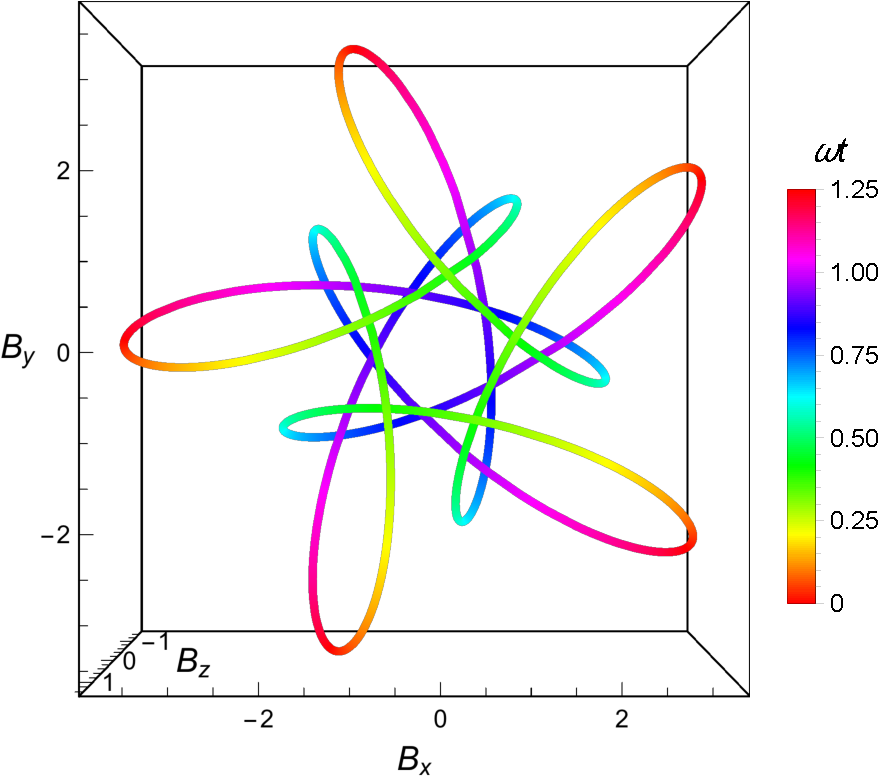
\includegraphics[width=9cm]{figures/5_2.pdf}
\caption{ (a)Parametric plot of a magnetic field $\ve{B}(t)$ with rotational symmetry of order $m=5$. The coefficient $a_0$ is set to zero (no static component); all other coefficients---$c_1$, $c_4$, $d_4$, $c_5$, $d_5$, $c_6$, and $d_6$---are set to 1. The color map shows the time $\omega t$ modulo $2\pi/m$, highlighting the 5-fold rotational symmetry.(b)The force balance on the magnetic roller on an inclined surface }
\label{fig:1}
\end{figure}
 
 \begin{figure}[p]
\centering
\includegraphics[width=9cm]{figures/5_3.pdf}
\caption{(a)the converge plot for the optimization process (b)optimized results of trajectory via the physics model model navigated to different directions   }
\label{fig:1}
\end{figure}
 \section{Results and Discussion}
 \begin{figure}[p]
\centering
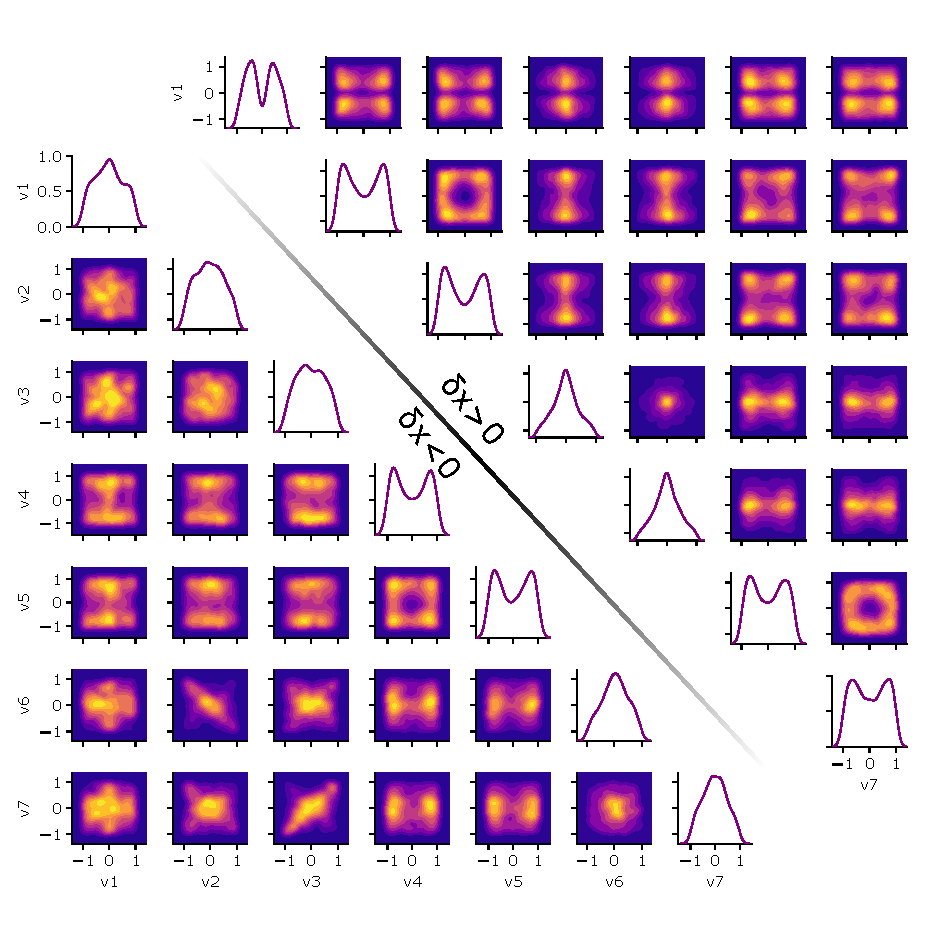
\includegraphics[width=9cm]{figures/5_4.pdf}
\caption{ Statistical study on the properties of navigation.(a)correlation between each design parameters in   (b) depend on the distance between spheres and surface (c) depend on the number of summery (d) depends on frequency (e) depend on the slope}
\label{fig:1}
\end{figure}
 \section{Preliminary experiment Results}
 \begin{figure}[p]
\centering
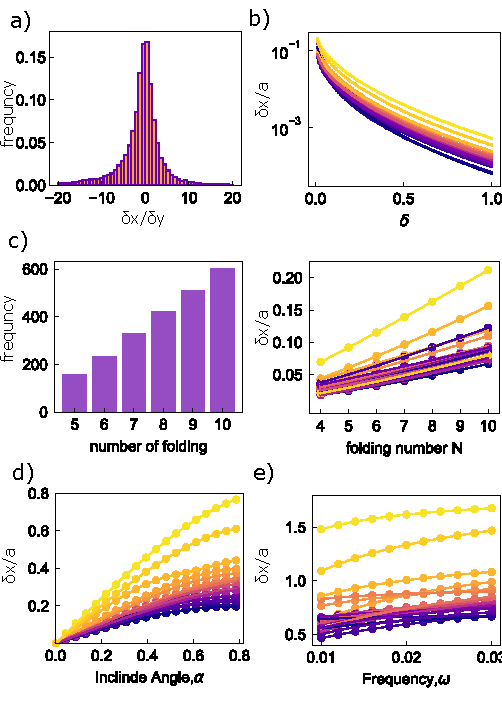
\includegraphics[width=9cm]{figures/5_5.pdf}
\caption{ (a) Experiment showing navigation into different direction (b) reveres the rotation reverse the navigation direction (c) on different slope (d)with different frequency  }
\label{fig:1}
\end{figure}
  \section{Conclusion}
